% Tài liệu bổ sung của paper_vi/main_vi.tex. Bảng số sinh tự động bởi tables/make_tables.py (không sửa tay).
\documentclass[11pt,a4paper]{article}
\usepackage[utf8]{inputenc}
\usepackage[T5]{fontenc}
\usepackage[vietnamese]{babel}
\usepackage[margin=2.5cm]{geometry}
\usepackage{amsmath,amssymb,booktabs,array,graphicx,xcolor}
\usepackage[colorlinks=true,linkcolor=blue]{hyperref}
\graphicspath{{../paper_en/figures/}{./}}
\newcommand{\Ntau}{N_{\tau}}
\newcommand{\todo}[1]{\textcolor{red}{[TODO: #1]}}
\renewcommand{\thetable}{S\arabic{table}}
\renewcommand{\thefigure}{S\arabic{figure}}
\title{Tài liệu bổ sung: Tấn công cạn kiệt tài nguyên qua NMS có thực sự làm chậm bộ phát hiện? Một nghiên cứu đo lường trên CPU ghim lõi}
\date{}
\begin{document}
\maketitle

\section{Bộ tối ưu của nghiên cứu tình huống}
Quy trình tối ưu và đánh giá miếng dán được tóm tắt ở Bảng~\ref{tab:algo}; thiết lập của từng điều kiện ở bài chính. Fitness huấn luyện theo ngân sách (Bảng~\ref{tab:train}, Hình~\ref{fig:budget}) cho thấy thuật toán di truyền bão hòa sớm và không vượt tìm kiếm ngẫu nhiên cùng cách đặt vị trí; baseline gradient (hộp trắng) cao hơn xa mọi điều kiện không dùng gradient. Giá trị fitness phụ thuộc vào ngưỡng và kích thước đầu vào, nên chỉ so được trong cùng đầu vào và ngưỡng.

\begin{table}[h]
\centering\small
\caption{Quy trình tối ưu và đánh giá miếng dán.}
\label{tab:algo}
\begin{tabular}{@{}cp{12.5cm}@{}}
\toprule
Bước & Thao tác \\
\midrule
1 & Khởi tạo 20 tensor RGB; chọn vị trí theo chính sách (độ nổi bật, tâm hoặc ngẫu nhiên). \\
2 & Chèn từng cá thể vào các ảnh tối ưu. \\
3 & Lấy mẫu biến đổi; suy luận và đọc điểm tin cậy trước NMS. \\
4 & Tính fitness; ghi số lượt ảnh và cá thể tốt nhất. \\
5 & Giữ năm cá thể ưu tú; lai ghép ngang và đột biến để tạo 15 con. \\
6 & Dừng khi hết ngân sách lượt ảnh; khóa miếng dán và ghi giá trị băm. \\
7 & Đánh giá độc lập trên ảnh giữ ra ngoài. \\
\bottomrule
\end{tabular}
\end{table}

% SINH TỰ ĐỘNG bởi paper_vi/tables/make_tables.py — KHÔNG SỬA TAY.
\begin{table}[t]
\centering\small
\caption{Fitness huấn luyện (trung bình trên mười seed, độ lệch chuẩn trong ngoặc) ở ba mức ngân sách (lượt lan truyền thuận ứng viên--ảnh), trường \texttt{best\_training\_fitness} của checkpoint. Với B4, phương pháp gradient cập nhật một patch duy nhất nên giá trị là fitness ở bước cuối của mốc ngân sách.}
\label{tab:train}
\begin{tabular}{@{}lccc@{}}
\toprule
Điều kiện & 10\,000 & 25\,000 & 62\,500 \\
\midrule
C1 (320 px, $\tau_{\mathrm{obj}}$ 0,01) & 185,1 (1,7) & 185,9 (1,2) & 186,6 (1,6) \\
C3 (320 px, $\tau_{\mathrm{obj}}$ 0,25) & 39,8 (0,2) & 40,0 (0,3) & 40,5 (0,3) \\
C2 (640 px, patch 128 px) & 294,4 (3,9) & 295,5 (2,9) & 297,3 (2,2) \\
C4 (640 px, patch 64 px) & 299,4 (1,3) & 301,4 (1,9) & 303,1 (1,7) \\
B1 (đặt ở tâm) & 188,7 (1,5) & 189,8 (1,0) & 191,0 (1,4) \\
B2 (đặt ngẫu nhiên) & 191,6 (1,9) & 193,1 (1,5) & 193,5 (1,9) \\
B3 (tìm kiếm ngẫu nhiên) & 184,5 (0,8) & 185,1 (0,8) & 186,0 (1,0) \\
B4 (gradient, tanh) & 218,1 (14,9) & 314,4 (12,8) & 334,1 (11,6) \\
\bottomrule
\end{tabular}
\end{table}


\begin{figure}[h]
\centering
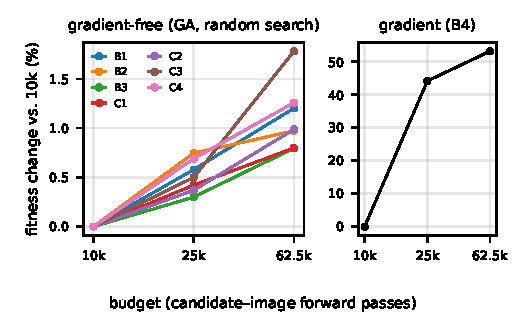
\includegraphics[width=0.8\textwidth]{fig7_training_budget.pdf}
\caption{Thay đổi fitness huấn luyện (trung bình mười seed) theo ngân sách, so với mốc 10\,000 lượt.}
\label{fig:budget}
\end{figure}

\section{Mô tả thêm của đối chứng dương}
Bảng~\ref{tab:slopes} cho độ dốc log--log của các đường cong đáp ứng liều; chỉ mang tính mô tả, không suy ra lớp độ phức tạp. Về số lớp: các cài đặt không phân biệt lớp không bị ảnh hưởng bởi số lớp, còn các cài đặt phân biệt lớp nhanh hơn khi chỉ có một lớp (số liệu: \texttt{contrasts.nc80\_over\_nc1} trong tệp tóm tắt của đối chứng dương).

% SINH TỰ ĐỘNG bởi paper_vi/tables/make_tables.py — KHÔNG SỬA TAY.
\begin{table}[t]
\centering\small
\caption{Độ dốc log--log của độ trễ NMS theo $\Ntau$ trên các mức đã đo $\ge 100$ (head 10\,000 anchor, 80 lớp, không giới hạn); khoảng tin cậy bootstrap 95\% trong ngoặc. Chỉ mang tính mô tả.}
\label{tab:slopes}
\begin{tabular}{@{}lccc@{}}
\toprule
Cách cài đặt & Rời nhau & Cụm dày đặc & Hỗn hợp \\
\midrule
PyTorch thuần & 1,17 [1,17; 1,17] & 0,30 [0,29; 0,32] & 1,07 [1,05; 1,08] \\
torchvision \texttt{nms} & 1,59 [1,58; 1,60] & 0,69 [0,67; 0,69] & 1,42 [1,40; 1,45] \\
torchvision theo lô & 1,09 [1,08; 1,10] & 1,08 [1,07; 1,09] & 1,07 [1,05; 1,08] \\
Ultralytics gốc & 1,29 [1,29; 1,30] & 0,96 [0,95; 0,97] & 1,21 [1,20; 1,21] \\
\bottomrule
\end{tabular}
\end{table}


\section{Tỷ số NMS theo cách cài đặt cho từng patch}
% SINH TỰ ĐỘNG bởi paper_vi/tables/make_tables.py — KHÔNG SỬA TAY.
\begin{table*}[t]
\centering\small
\caption{Tỷ số thời gian công đoạn NMS của ảnh có patch so với ảnh sạch cùng canvas tại $\tau=0{,}01$ (tỷ số trung bình, KTC 95\% bootstrap hai tầng), theo cách cài đặt; cùng lần đo lại patch (bước chèn ngoài vùng bấm giờ) với bảng patch của bài chính.}
\label{tab:impl}
\begin{tabular}{@{}lcccc@{}}
\toprule
Điều kiện & PyTorch thuần & \texttt{nms} & Theo lô & Ultralytics \\
\midrule
\multicolumn{5}{c}{\todo{E11 chưa đo: chạy studies/e11\_patch\_remeasure rồi chạy lại make\_tables.py}} \\
\bottomrule
\end{tabular}
\end{table*}


\section{Kiểm tra chéo, post hoc: lần đo patch trước có lỗi chèn patch}
Lần đo patch trước (studies/e6\_remeasure) gọi bước chèn patch bên trong vùng bấm giờ của nhánh có patch nhưng không gọi ở nhánh sạch. Bảng~\ref{tab:supp_corrected} giữ số gốc và một phép hiệu chỉnh bằng phép trừ, với chi phí chèn đo ở một phiên chẩn đoán khác. Đây chỉ là kiểm tra chéo; kết quả chính là lần đo lại với bước chèn ngoài vùng bấm giờ (bài chính, Bảng patch). Mọi bản ghi thô của lần đo trước được giữ.

% SINH TỰ ĐỘNG bởi paper_vi/tables/make_tables.py — KHÔNG SỬA TAY.
\begin{table}[t]
\centering\small
\caption{\textbf{Kiểm tra chéo, post hoc.} Lần đo patch trước (E6/E6-A1/E6-A2) tính bước chèn patch trong vùng bấm giờ chỉ ở nhánh có patch. Cột ``chưa hiệu chỉnh'' là tỷ số gốc; cột ``hiệu chỉnh'' cộng chi phí chèn đo ở một phiên khác (320px_patch64: 0,354~ms, 640px_patch128: 1,658~ms, 640px_patch64: 0,534~ms) vào mẫu số. Không dùng làm kết quả chính; kết quả chính là lần đo lại trong bảng patch của bài chính.}
\label{tab:supp_corrected}
\begin{tabular}{@{}llcc@{}}
\toprule
Điều kiện & Cách cài đặt & Chưa hiệu chỉnh & Hiệu chỉnh \\
\midrule
C1 (320 px) & torchvision \texttt{nms} & 1,013 (1,006--1,021) & 1,006 (0,999--1,014) \\
C1 (320 px) & PyTorch thuần & 1,007 (0,994--1,018) & 1,000 (0,988--1,011) \\
C3 (320 px) & torchvision \texttt{nms} & 1,015 (1,007--1,025) & 1,008 (1,000--1,018) \\
C3 (320 px) & PyTorch thuần & 1,008 (0,996--1,019) & 1,002 (0,989--1,012) \\
B1 (320 px) & torchvision \texttt{nms} & 1,010 (1,002--1,020) & 1,003 (0,995--1,012) \\
B1 (320 px) & PyTorch thuần & 1,004 (0,991--1,016) & 0,997 (0,984--1,009) \\
B2 (320 px) & torchvision \texttt{nms} & 1,012 (1,005--1,022) & 1,005 (0,997--1,014) \\
B2 (320 px) & PyTorch thuần & 1,005 (0,993--1,015) & 0,998 (0,986--1,008) \\
B3 (320 px) & torchvision \texttt{nms} & 1,011 (1,003--1,019) & 1,003 (0,996--1,012) \\
B3 (320 px) & PyTorch thuần & 1,006 (0,994--1,017) & 0,999 (0,987--1,010) \\
B4 (320 px) & torchvision \texttt{nms} & 1,008 (1,002--1,015) & 1,001 (0,994--1,007) \\
B4 (320 px) & PyTorch thuần & 1,022 (1,010--1,033) & 1,015 (1,003--1,025) \\
C2 (640 px) & torchvision \texttt{nms} & 1,011 (1,005--1,016) & 1,001 (0,995--1,006) \\
C2 (640 px) & PyTorch thuần & 1,008 (1,002--1,014) & 0,998 (0,992--1,004) \\
C4 (640 px) & torchvision \texttt{nms} & 1,012 (1,005--1,019) & 1,009 (1,002--1,016) \\
C4 (640 px) & PyTorch thuần & 1,014 (1,006--1,022) & 1,011 (1,003--1,018) \\
\bottomrule
\end{tabular}
\end{table}


\end{document}
